\documentclass[tikz,border=8pt]{standalone}
\usepackage{amsmath}
\usepackage{amssymb}
\usetikzlibrary{arrows.meta,calc,positioning}

\definecolor{basisblue}{HTML}{2F6F9F}
\definecolor{basisgreen}{HTML}{5F7F55}
\definecolor{basisgold}{HTML}{A66F00}
\definecolor{textgray}{HTML}{2F3437}
\definecolor{linegray}{HTML}{AEB7BC}
\definecolor{softgray}{HTML}{F5F7F8}

\begin{document}
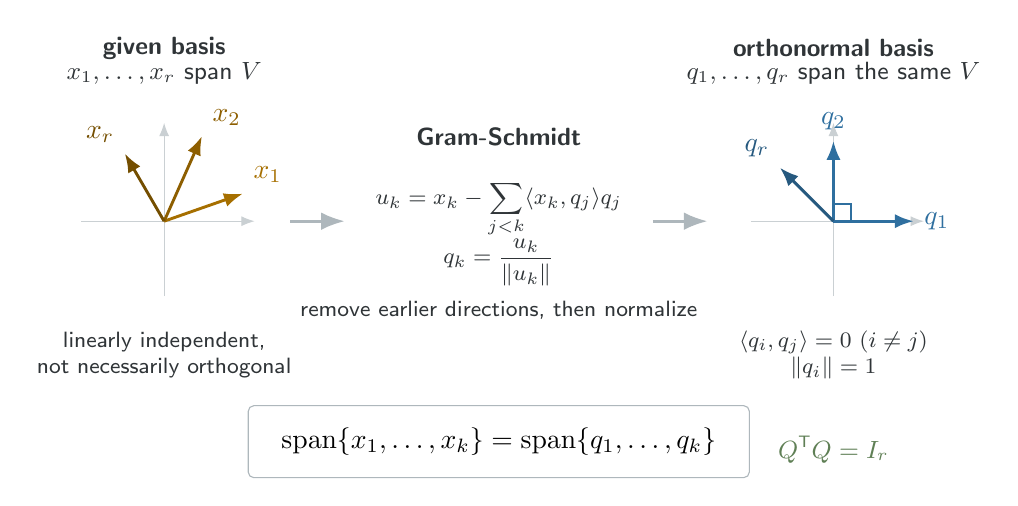
\begin{tikzpicture}[
  font=\sffamily,
  >=Latex,
  vector/.style={-{Latex[length=2.4mm]}, line width=1.05pt},
  maparrow/.style={-{Latex[length=3mm]}, line width=1.0pt, draw=linegray},
  stage/.style={
    draw=linegray,
    fill=softgray,
    rounded corners=2pt,
    inner xsep=12pt,
    inner ysep=8pt,
    align=center
  },
  label/.style={font=\sffamily\bfseries\small, text=textgray},
  smallnote/.style={font=\sffamily\small, text=textgray, align=center},
  mathnote/.style={font=\sffamily\footnotesize, text=textgray, align=center}
]

% Left: original basis.
\node[label] at (-4.25, 2.35) {given basis};
\node[smallnote] at (-4.25, 2.03) {$x_1,\ldots,x_r$ span $V$};

\coordinate (O) at (-4.25, 0.15);
\draw[->, draw=linegray!65] ($(O)+(-1.05,0)$) -- ($(O)+(1.15,0)$);
\draw[->, draw=linegray!65] ($(O)+(0,-0.95)$) -- ($(O)+(0,1.25)$);
\draw[vector, draw=basisgold] (O) -- ++(1.00,0.35) node[anchor=south west, text=basisgold] {$x_1$};
\draw[vector, draw=basisgold!85!black] (O) -- ++(0.48,1.08) node[anchor=south west, text=basisgold!85!black] {$x_2$};
\draw[vector, draw=basisgold!70!black] (O) -- ++(-0.50,0.86) node[anchor=south east, text=basisgold!70!black] {$x_r$};
\node[mathnote] at (-4.25,-1.55) {linearly independent,\\not necessarily orthogonal};

% Center: Gram-Schmidt step.
\node[minimum width=3.9cm, minimum height=2.8cm, inner sep=0pt] (gs) at (0,0.15) {};
\node[label] at (gs.north) [yshift=-0.33cm] {Gram-Schmidt};
\node[mathnote] at (0,0.30) {$u_k=x_k-\displaystyle\sum_{j<k}\langle x_k,q_j\rangle q_j$};
\node[mathnote] at (0,-0.37) {$q_k=\dfrac{u_k}{\lVert u_k\rVert}$};
\node[mathnote] at (0,-0.98) {remove earlier directions, then normalize};

% Right: orthonormal basis.
\node[label] at (4.25, 2.35) {orthonormal basis};
\node[smallnote] at (4.25, 2.03) {$q_1,\ldots,q_r$ span the same $V$};

\coordinate (Q) at (4.25, 0.15);
\draw[->, draw=linegray!65] ($(Q)+(-1.05,0)$) -- ($(Q)+(1.15,0)$);
\draw[->, draw=linegray!65] ($(Q)+(0,-0.95)$) -- ($(Q)+(0,1.25)$);
\draw[vector, draw=basisblue] (Q) -- ++(1.02,0) node[anchor=west, text=basisblue] {$q_1$};
\draw[vector, draw=basisblue] (Q) -- ++(0,1.02) node[anchor=south, text=basisblue] {$q_2$};
\draw[vector, draw=basisblue!80!black] (Q) -- ++(-0.68,0.68) node[anchor=south east, text=basisblue!80!black] {$q_r$};
\draw[draw=basisblue, line width=0.7pt] ($(Q)+(0.22,0)$) -- ++(0,0.22) -- ++(-0.22,0);
\node[mathnote] at (4.25,-1.55) {$\langle q_i,q_j\rangle=0\ (i\ne j)$\\$\lVert q_i\rVert=1$};

% Flow arrows and invariant.
\draw[maparrow] (-2.65,0.15) -- (gs.west);
\draw[maparrow] (gs.east) -- (2.65,0.15);

\node[stage, fill=white, minimum width=3.55cm] at (0,-2.65)
  {$\operatorname{span}\{x_1,\ldots,x_k\}=\operatorname{span}\{q_1,\ldots,q_k\}$};

\node[smallnote, text=basisgreen] at (4.25,-2.75) {$Q^\mathsf{T}Q=I_r$};

\end{tikzpicture}
\end{document}
